\chapter{On-Wire Protocol}
\label{section-8}

The heart of the NTP on-wire protocol is the core mechanism that
exchanges time values between servers, peers, and clients. It is
inherently resistant to lost or duplicate packets. Data integrity is
provided by the IP and UDP checksums. No flow control or
retransmission facilities are provided or necessary. The protocol
uses timestamps, which are either extracted from packet headers or
struck from the system clock upon the arrival or departure of a
packet. Timestamps are precision data and should be restruck in the
case of link-level retransmission and corrected for the time to
compute a MAC in transmit.

NTP messages make use of two different communication modes, one-to-
one and one-to-many, commonly referred to as unicast and broadcast.
For the purposes of this document, the term broadcast is interpreted
as any available one-to-many mechanism. For IPv4, this equates to
either IPv4 broadcast or IPv4 multicast. For IPv6, this equates to
IPv6 multicast. For this purpose, IANA has allocated the IPv4
multicast address 224.0.1.1 and the IPv6 multicast address ending
:101, with the prefix determined by scoping rules. Any other non-
allocated multicast address may also be used in addition to these
allocated multicast addresses.

The on-wire protocol uses four timestamps numbered $ t1 $ through $ t4 $ and
three state variables org, rec, and xmt, as shown in Figure~\ref{on_wire_protocol}. This
figure shows the most general case where each of two peers, $ A $ and $ B $,
independently measure the offset and delay relative to the other.
For purposes of illustration, the packet timestamps are shown in
lowercase, while the state variables are shown in uppercase. The
state variables are copied from the packet timestamps upon arrival or
departure of a packet.

\begin{figure}
\centering
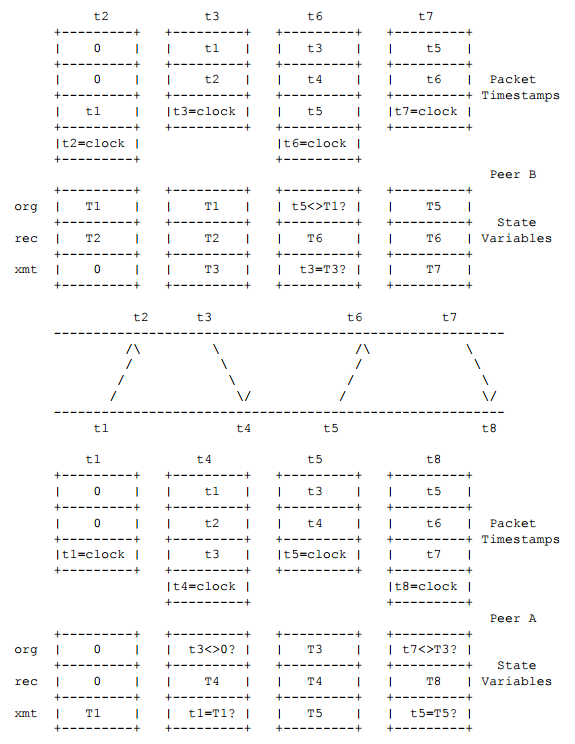
\includegraphics[width=\textwidth]{on_wire_protocol.png}
\caption{On-Wire Protocol}
\label{on_wire_protocol}
\end{figure}

In the figure, the first packet transmitted by $ A $ contains only the
origin timestamp $ t1 $, which is then copied to $ T1 $. $ B $ receives the
packet at $ t2 $ and copies $ t1 $ to $ T1 $ and the receive timestamp $ t2 $ to $ T2 $.
At this time or some time later at $ t3 $, $ B $ sends a packet to $ A $
containing $ t1 $ and $ t2 $ and the transmit timestamp $ t3 $. All three
timestamps are copied to the corresponding state variables. $ A $
receives the packet at $ t4 $ containing the three timestamps $ t1 $, $ t2 $, and
$ t3 $ and the destination timestamp $ t4 $. These four timestamps are used
to compute the offset and delay of $ B $ relative to $ A $, as described
below.

Before the xmt and org state variables are updated, two sanity checks
are performed in order to protect against duplicate, bogus, or
replayed packets. In the exchange above, a packet is duplicate or
replay if the transmit timestamp $ t3 $ in the packet matches the org
state variable $ T3 $. A packet is bogus if the origin timestamp $ t1 $ in
the packet does not match the xmt state variable $ T1 $. In either of
these cases, the state variables are updated, then the packet is
discarded. To protect against replay of the last transmitted packet,
the xmt state variable is set to zero immediately after a successful
bogus check.

The four most recent timestamps, $ T1 $ through $ T4 $, are used to compute
the offset of $ B $ relative to $ A $

$$
\theta = T(B) - T(A) = \frac{1}{2} \cdot ((T2 - T1) + (T3 - T4))
$$

and the round-trip delay

$$
\delta = T(ABA) = (T4 - T1) - (T3 - T2).
$$

Note that the quantities within parentheses are computed from 64-bit
unsigned timestamps and result in signed values with 63 significant
bits plus sign. These values can represent dates from 68 years in
the past to 68 years in the future. However, the offset and delay
are computed as sums and differences of these values, which contain
62 significant bits and two sign bits, so they can represent
unambiguous values from 34 years in the past to 34 years in the
future. In other words, the time of the client must be set within 34
years of the server before the service is started. This is a
fundamental limitation with 64-bit integer arithmetic.

In implementations where floating double arithmetic is available, the
first-order differences can be converted to floating double and the
second-order sums and differences computed in that arithmetic. Since
the second-order terms are typically very small relative to the
timestamp magnitudes, there is no loss in significance, yet the
unambiguous range is restored from 34 years to 68 years.

In some scenarios where the initial frequency offset of the client is
relatively large and the actual propagation time small, it is
possible for the delay computation to become negative. For instance,
if the frequency difference is 100 ppm and the interval $ T4 - T1 $ is 64
s, the apparent delay is -6.4 ms. Since negative values are
misleading in subsequent computations, the value of delta should be
clamped not less than s.rho, where s.rho is the system precision
described in Section~\ref{section-11-1}, expressed in seconds.

The discussion above assumes the most general case where two
symmetric peers independently measure the offsets and delays between
them. In the case of a stateless server, the protocol can be
simplified. A stateless server copies $ T3 $ and $ T4 $ from the client
packet to $ T1 $ and $ T2 $ of the server packet and tacks on the transmit
timestamp $ T3 $ before sending it to the client. Additional details for
filling in the remaining protocol fields are given in a Section~\ref{section-9} and
following sections and in the appendix.

Note that the on-wire protocol as described resists replay of a
server response packet. However, it does not resist replay of the
client request packet, which would result in a server reply packet
with new values of $ T2 $ and $ T3 $ and result in incorrect offset and
delay. This vulnerability can be avoided by setting the xmt state
variable to zero after computing the offset and delay.
